\documentclass[12pt]{IEEEtran}
\usepackage[T1]{fontenc}
%\documentclass[12pt]{Article}
%\renewcommand\rmdefault{phv}
%\usepackage[doublespacing]{setspace}
%\usepackage[margin=1in]{geometry}
\usepackage{hyperref}
\usepackage{graphicx}
\usepackage{amsmath}
\usepackage{pgfplots}
\usepackage{hyperref}
\usepackage{breakurl}
\usepackage{indentfirst}
\usepackage{authblk}
\usepackage{todonotes}
\usepackage{svg}


\usepackage[backend=biber]{biblatex}
\addbibresource{ZTree.bib}

\title{Z-Table: A Novel Range-Queryable Distributed Data Structure for Use in P2P Sensornets}
\author{Siemen's Competition 2015}
\date{\vspace{-5ex}}

\begin{document}

\maketitle

\begin{abstract}
We present the design and implementation of a novel data structure (the 'Z-Table'). We aim to solve the issue of window/range-based queries in peer to peer architectures. Traditional models, for example,  distributed hash tables (DHT), are hostile towards window queries because their hashing operations are designed to uniformly distribute stored data across a defined key space; the hashing operations used to achieve this pseudo-random distribution inherently erases all characteristics of the target data that could be used to define locality. We solve this problem of erasure by defining a scheme in which higher-order data is mapped to a first-dimensional key space, while preserving locality. The resulting keys pace is very definitely not uniformly distributed, so we define a distributed consensus scheme in which participants in our Z-Tables agree to target highly populated regions of the key space. This consensus scheme also provides some protection from Sybil attacks. Finally, we define storage, lookup, and deletion operations that utilize balanced search trees to efficiently perform necessary network functions; the preservation of locality allows us to greatly optimize these operations through the use of balanced trees. A peer to peer communication system acts as the underlying network for participants, providing all of the traditional benefits of a P2P architecture (scalability, robustness, etc.).
\end{abstract}


\section{Notation}

\noindent Tuples/Lists: $[a,b,c,...]$

\noindent Application of a function $f$ to an input $x$: $y=f(x)$

\noindent Application of a hash function $H$ with $k$ output bits: $H_{k}(x) = \{0,1\}^k$

\noindent Keys of user $j$: $ PUBK_j; PRIVK_j $

 
\section{Introduction}
\par Distributed hash tables are currently one of the hottest topics in the cryptography space~\cite{Stoica:2001dj,Rowstron:2001ea,Ratnasamy:2001wn}. They are used in many large scale open sources projects~\cite{Freitas:2013tb,Xu:2010vs,Perfitt:2010fh} as their underlying infrastructure. First, in order to better understand the motivation behind this project, a brief explanation of the workings of a distributed has table (DHT) and its constituent protocols is needed.

\par Simply put, DHTs were created to provide hash table-like functionality on an Internet-scale level~\cite{Ratnasamy:2001wn}. They expose basic PUT and GET requests (operating on (key,value) pairs) to clients, allowing them to store and retrieve information from the DHT. The difference between a hash table and a DHT is the scope of the mechanism: DHTs are able to operate in an entirely decentralized setting, in which the responsibility for the mapping of keys to values is distributed pseudo-uniformly among all participants in a P2P network. Notable networks that utilize DHTs include the Coral Content Distribution Network~\cite{Freedman:2004vb}, the Storm Botnet~\cite{Holz:2008uk}, and the BitTorrent file sharing protocol~\cite{Cohen:y1_8mBnw}.

\par Keys used in traditional DHTs are calculated through the use of a hash function. Given that the digest (output) of a hash function is some number of bits, each of which has the same probability of being set to $'1'$ or $'0'$, we can confidently conclude that the outputs will be randomly distributed along the hash function's key space~\todo{citation}. This keyspace is the set of all possible outputs; for a hash function with $k$ output bits, this is the set $\{0,1\}^k$. This is useful to users in a DHT because, assuming that a given hash function is 'sound,' in that its outputs are actually evenly distributed, they are able to mathematically verify the even partitioning of the key space. The participants can thus trust that the load will be balanced fairly among all nodes. No one node will have complete control, and no group of nodes will be unfairly burdened due to their residing in some supposed 'hotspots' in the key space, in which a disproportionally high number of objects are stored.~\todo{citations?}

\par One important continuity between all of these examples is the use of a DHT in an 'exact-match' lookup scenario; the even distribution of hash functions once again comes into play. The purging of any locality (that is, the property of alike object's digests being somehow as 'distant' from one another as the objects themselves) precludes the possibility of range or window-based queries. Ramabhadran et al.~\todo{cite} put it very well: \textit{"However, range queries, asking for all objects with values in a certain range, are particularly difficult to implement in DHTs. This is because DHTs use hashing to distribute keys uniformly and so can't rely on any structural properties of the key space, such as an ordering among keys."}



The idea of locality vs. evenness is fundamental to our work, and so we define it here. Intuitively, we can say that locality is preserved for any given set of objects (serializable to a numeric representation in some fashion) $A,B,$ and $C$ in a function $f$ such that
\begin{equation}
|A-B| < |B-C| \Rightarrow |f(A)-f(B)| < |f(B) - f(C)|,
\end{equation}
and garden variety hash functions obviously do not fulfill this requirement.

\par Some research has been done on the usage of a DHT as an overlay on top of a traditional data structure to enable range queries\todo{cite skiptree and DST}, however none of the currently proposed solutions are useful in a true P2P network. Sybil attacks are arguably the most severe vulnerability in most decentralized networks~\todo{cite}, with a litany of papers having been published on this attack in the context of DHTs~\todo{cite}, and yet the subject is not even broached.

\par Given that if we replace the cryptographic hash function in a DHT with a locality sensitive function~\footnote{Locality sensitive hash functions do exist, however we believe that a lower level function, such as a generic space filling curve, would be better suited for our purpose.}, the distribution of keys along the key space will not be even, and so we must design a scheme by which nodes can coalesce onto the more populated areas.

\par A DHT that satisfies all of these requirements would be extremely helpful to users in a variety of settings. Sensornets have been the darling of the P2P research and usage communities for some time now, and we believe that our data structure could allow for distributed sensornets in which both the collection \textit{and} the lookup/analysis processes are decentralized. To be clear, no other data structure in existence has these capabilities. In fact, this work is the direct result of an inability to find an existing solution. Some potential applications include:



\section{Proposed Solution}
\begin{figure}[!t]
\centering
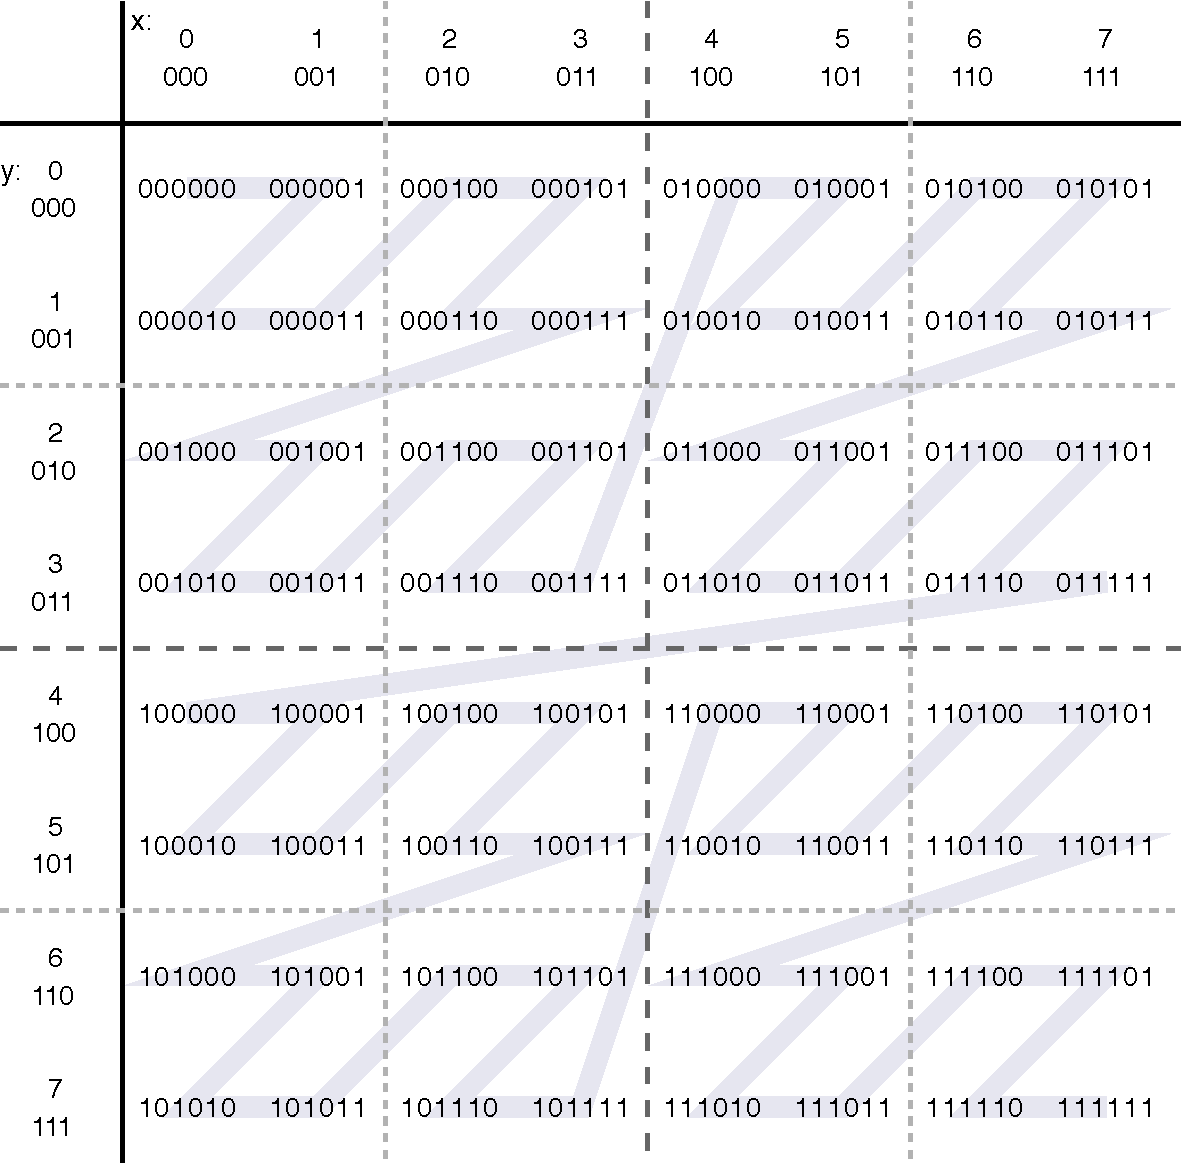
\includegraphics[width=3in]{ZCurve}
\caption{Bit Interleaving With A Z Order Curve}
\label{fig_ZOrd}
\end{figure}

\par We believe that the best solution is one in which we only slightly modify the way in which a DHT works. Substituting a space filling curve for a hash function would allow us to preserve locality of data in a DHT with rigorously defined limitations on what kind of data may be stored in it.

\par Currently, we believe that bit interleaving is a promising replacement for hash functions.



\printbibliography
\end{document}
